\documentclass{article}
\usepackage{graphicx}
\usepackage{mathtools}
\usepackage{xfrac}
\usepackage{amsmath, amssymb}
\usepackage{listings}
\usepackage{float}
\usepackage{wrapfig}
\usepackage{tikz}
\usepackage{fullpage}
\usepackage{hyperref}
\usepackage{mathalpha}
\usepackage{tikz}
\usepackage{cite}
\usepackage{amsthm}

\newtheorem{theorem}{Proposition}[section]
\newtheorem{corollary}{Corollary}[theorem]
\newtheorem{lemma}[theorem]{Lemma}

\theoremstyle{definition}
\newtheorem{definition}{Definition}[section]

\theoremstyle{remark}
\newtheorem*{remark}{Remark}
\newtheorem*{example}{Example}
\newtheorem*{notation}{Notation}

\title{Computational Simulation: Numerical Methods\\Assignment 2}
\author{David Lawton\\22337087}
\date{13th Oct. 2024.}

\begin{document}

\maketitle

\tableofcontents

\section{Introduction}
In this report we detail our analysis of the growth of human population since 1750, using an exponential growth model.\\
\indent The data we used was obtained from both `Gapminder' (1750 - 1940) and the `United States Census Bureau' (1950 - 2016).\\

\section{Exponential Growth Model}
The first step in our analysis was to view the data on a logarithmic scale with respect to population, as this would allow us to determine whether the growth of the human population was approximately exponential.\\
\indent Instead of a `passive' logarithmic transformation, where we change the scale on the plot, we ran an `active' logarithmic transformation on the data, where we took the natural logarithm of the population before plotting was done. This is done so that a linear regression can be applied to the transformed data, rather than an exponential one on the original data.\\
\subsection{Theory} 
In an exponential model the data is assumed to follow the form
\begin{equation}
    n(t) = n_0 \exp{[\lambda (t-t_0)]}
\end{equation}
which after our logarithmic transformation, becomes
\begin{equation}
    \ln{n(t)} = \ln{n_0} + \lambda (t-t_0)
\end{equation}
thus on our logarithmic plot, the transformed data follows a linear form.
\begin{equation}
    f(t) = \ln{n(t)} = a + b t
\end{equation}
where $a = \ln{n_0} - \lambda t_0$, $b = \lambda$.\\
\indent We now run a linear regression on subsets of the transformed data, which appear linear, to determine approximate values of $a_i$ and $b_i$, in the $i^{th}$ subset.\\
\begin{figure}[H]
    \centering
    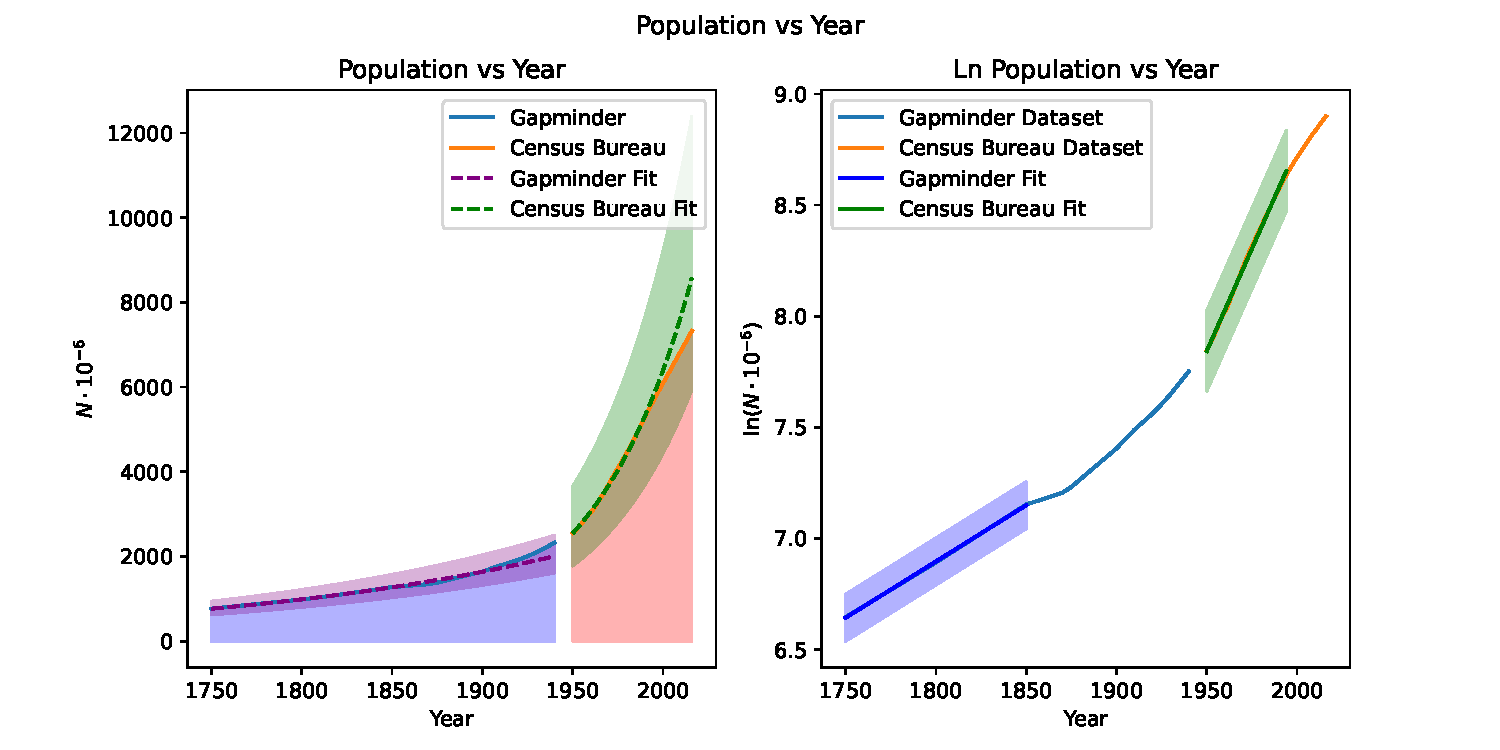
\includegraphics[width=\textwidth]{population_growth.pdf}
    \caption{\label{fig: Logarithmicplot} Plots of Population and natural log of population against time, with the exponential growth fit plotted with approx. 65\% confidence intervals in both. Note that the data is contained inside the confidence intervals, but does not follow the fit exactly.}
\end{figure}
\section{Results}
From our fit we obtained the following values for $a$ and $b$, in each subset\\

\begin{center}
\begin{tabular}{c|c|c|c|c}
    \hline
    \hline
    Subset $i$ & $a_i$ & $b_i$ & $\sigma_{a}$ & $\sigma_{b}$ \\ 
    \hline
    Subset 1 & -2.213 & 0.005061 & 0.1056 & 5.85e-05 \\ 
    Subset 2 & -28.01 & 0.01839 & 0.1818 & 9.22e-05 \\
    \hline
    \hline
\end{tabular}
\end{center}

This gives us the corresponding values for $n_0$ and $\lambda$, where $n_0$ is the population at $t_0$ for each subset, and $\lambda$ is the exponential growth rate.\\
\begin{center}
\begin{tabular}{c|c|c|c|c}
    \hline
    \hline
    Subset $i$ & $n_0$ & $\lambda$ & $\sigma_{n_0}$ & $\sigma_{\lambda}$ \\ 
    \hline
    Subset 1 & 768.0 & 0.005061 & 113.0 & 5.85e-05 \\ 
    Subset 2 & 2.55e+03 & 0.01839 & 651.9 & 9.22e-05 \\
    \hline
    \hline
\end{tabular}
\end{center}
Clearly, from figure \ref{fig: Logarithmicplot}, while the total dataset is within the margin of error of the fit of the subset, the data does seem to lag below the perfect exponential. This is because, effectively, the other variables determining population growth which are assumed to have, on aggregate, no effect in this model ($\lambda$ constant), are not constant.\\
\indent In terms of assessing a `current' population evolution, the fit is likely not very helpful. A more accurate method would perhaps be a machine learning model, using interpolation to increase the dataset size, and modelling many smaller systems (countries, continents) to gain a greater insight into the correlation of population growth with various other variables (GDP, war, education, quality of life, access to medicine, \dots).\\
\indent A more rudimentary method would be to use this model, but to fit some functions (exponential, power law, sigmoidal,  \dots) to the $\lambda$ values, to examine how the growth rate may change in the future. Of course in this case, $n_0$ is the current population, and $t_0$ is the current year.\\
\indent In this fashion we made a basic example, setting the current year to 2016, and the current population to the last value in the data. We then fitted a linear function to the $\lambda$ values, and projected values until 2030.\\

\begin{figure}[H]
    \centering
    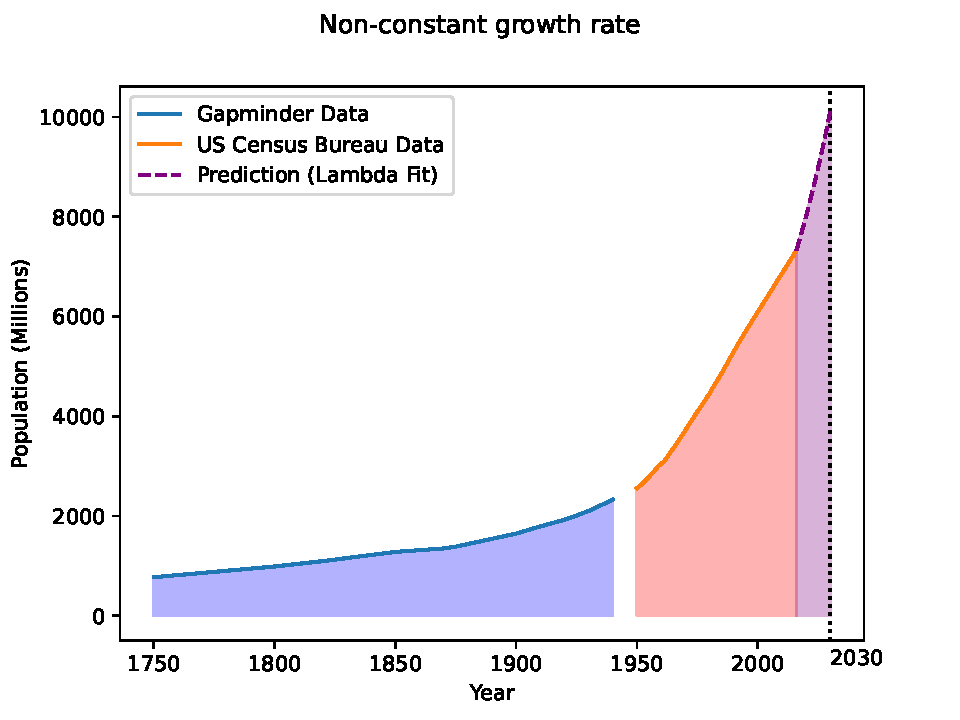
\includegraphics[width=0.8\textwidth]{non_constant_growth.pdf}
    \caption{\label{fig: Nonconstantgrowth} Plot of the predicted population growth until 2030, as marked, using the linear fit of the $\lambda$ values. While this is a slight overshoot as of 2022 world population data, it is a reasonable estimate, which would only be made more accurate by a larger dataset.}
\end{figure}

\textbf{I would like to mention that while GitHub Copilot was used to assist in the coding involved, it was used exclusively to autofill parts already written for other subsets, and answer questions regarding errors, and not to generate `new' code itself, nor text for this report.}

\end{document}